% !TeX root = ../../tfg.tex
% !TeX encoding = utf8
%
%*******************************************************
% Metodología
%*******************************************************

\chapter{Metodología}
\label{ch00:methodology}
La planificación y organización es un componente vital a la hora del desarrollo de software 
y la ciencia de datos, por lo que no es de extrañar que sus beneficios sean extrapolables
a otras áreas de la ciencia; 
hemos aplicado por ende la 
metodología expuesta en el artículo \cite{DBLP:journals/corr/abs-2104-12545}, realizado 
el trabajo con una mentalidad ágil, de acorde a las siguientes hipótesis: 

\begin{enumerate}
    \item Se premia la \textbf{reproducibilidad}, \textit{la ciencia no puede ser ciencia si no es reproducible}. Es por 
    ello que se publica todo el material usado. 
    \item \textbf{Comprobaciones} en todo los niveles, \textit{el código que no se ha probado no funciona}. 
    Explicitamos unos requisitos y criterios claros de validación. 
    \item Conocimiento libre, tanto la memoria como el código se encuentra publicado y con licencia libre en \href{https://github.com/BlancaCC/TFG-Estudio-de-las-redes-neuronales}{nuestro repositorio 
    de GitHub} \footnote{Puede visitarlo en \url{https://github.com/BlancaCC/TFG-Estudio-de-las-redes-neuronales}.}.
    \item \textbf{Colaboración frente jerarquía de mando vertical}, los tutores en este caso 
    los \textit{interesados en el producto} 
    indican qué les gustaría que tuviera en vez de un qué y cómo estricto. Consiguiendo con ello una mayor autonomía y bienestar de trabajo.
     
\end{enumerate}  

% Nota margen enfoque de la metodología 
\marginpar{\maginLetterSize
    \iconoAclaraciones \textcolor{dark_green}{     
        \textbf{
        El objetivo de la metodología seleccionada.
        }
    }

    Buscamos organizarnos de una manera eficiente con el fin de optimizar el proceso de producción y conducir a un resultado exitoso. Para ello nos basaremos en: 
    
    1.¿Qué personas se beneficiarán y están involucradas en el proyecto? (\textbf{Personas definidas } \ref{ch:metodología_personas})
    
    2.¿Qué caracteriza a esas personas y cuáles son sus necesidades? (\textbf{Historias de usuario} \ref{ch:metodología_personas_historias_de_usuario})
     
    3.¿Qué acciones satisfarán tales requisitos?(\textbf{Hitos} \ref{ch00:hitos})
   
}

Concretamente la metodología seguida basada en \cite{que-es-un-trabajo-fin-de-x} ha sido la siguiente: 


El objetivo es \textit{optimizar el proceso de diseño, entrenamiento y explotación}
para reducir su coste de cómputo 
y espacio en memoria en base de
un fundamento matemático sólido y sistemático que provenga de
la noción más elemental de red neuronal y no meras heurísticas experimentales.

Puesto que los problemas surgen de las necesidades humanas,
se han definido unas metas claras a través de la \textit{metodología de personas} 
(ver sección \ref{ch:metodología_personas}) \cite{personas-why-and-how-you-should-use-them}
y las respectivas historias de usuario derivadas (ver sección \ref{ch:metodología_personas_historias_de_usuario}).   

\section{\textit{Personas definidas}}  \label{ch:metodología_personas}

Ante la pregunta de quiénes serán los beneficiados e involucrados por este proyecto y que trataremos de satisfacer
han surgido 
las siguientes \textit{personas ficticias}:

\begin{itemize}

    \item \textbf{Rosa Camarero}, desea implementar un modelo de red neuronal que mejore a los actuales en algún aspecto, ya sea porque reduzca su coste computacional o espacio en memoria. 

    \item \textbf{María López}, catedrática en matemáticas aplicadas y miembro del tribunal. Su conocimiento
    de informática es moderado. Valora una memoria formal y rigurosa. Se encarga de evaluar trabajos fin de grado, en particular éste mismo.
    
    \item \textbf{Pedro Castillo}, Doctor experto en \textit{deep learning} y miembro del tribunal. Valora la claridad, las experimentaciones sensatas y fundamentadas así como la posibilidad de aplicaciones reales. Se encarga de evaluar trabajos fin de grado, en particular éste mismo. 
    
    \item \textbf{Javier Merí}, profesor del departamento de análisis matemático y contutor del proyecto (junto con JJ). Busca de manera formal y rigurosa entender y optimizar las redes neuronales usando herramientas analíticas. Estará presente durante todo el desarrollo. 
    
    \item   \textbf{JJ Merelo}, profesor del departamento de arquitectura de computadores y contutor del proyecto (junto con Javier). 
    Busca resolver problemas relacionados con la optimización bajo un punto de vista más práctico y experimental, salvaguardando un trabajo bien organizado y metódico. Estará presente durante todo el desarrollo. 

    \item \textbf{Blanca Cano} alumna de informáticas y matemáticas, tiene muchas ganas de aprender sobre redes 
    neuronales, su conocimiento es moderado, espera presentar el trabajo en la convocatoria ordinaria. 

\end{itemize}

\section{Historias de usuario}   \label{ch:metodología_personas_historias_de_usuario}

A partir de los usuarios se han definido las historias de usuario \cite{UserStories}, que han quedado registradas 
como \textit{issues} etiquetadas con \textit{user story} y cabecera de formato
\texttt{[HUxx] título de la historia de usuario}  en \href{https://github.com/BlancaCC/TFG-Estudio-de-las-redes-neuronales}{nuestro repositorio 
de GitHub},
 donde \texttt{HUxx} representa
la historia de usuario número $xx$.   

Las historias de usuario definidas son las siguientes: 

\subsubsection*{\href{https://github.com/BlancaCC/TFG-Estudio-de-las-redes-neuronales/issues/48}{[HU01] Optimización redes neuronales.}
}\label{HU01}
    Como \textit{Rosa} me gustaría que se ejecutaran las redes neuronales en un hardware
    más barato o que consuma menos en un tiempo razonable.
 
\subsubsection*{ \href{https://github.com/BlancaCC/TFG-Estudio-de-las-redes-neuronales/issues/65}{[HU02] Metodología}
} \label{HUO2}

Como \textit{JJ} me gustaría que el proyecto se realizara bajo un desarrollo ágil,  el cual recoge sus principios en el siguiente manifiesto \cite{principios-manifiesto-agil} y que es una filosofía, no una metodología \cite{why-agile-is-not-a-methodology-1} \cite{why-agile-is-not-a-methodology-2}.
Puede encontrar su declaración en las historias de usuario definidas en \href{https://github.com/BlancaCC/TFG-Estudio-de-las-redes-neuronales}{nuestro repositorio 
de GitHub} \footnote{Visite el \textit{issue} 65 \url{https://github.com/BlancaCC/TFG-Estudio-de-las-redes-neuronales/issues/65}.}.
 

\subsubsection*{ 
    \href{https://github.com/BlancaCC/TFG-Estudio-de-las-redes-neuronales/issues/50}{
    [HU03] Estudio de las redes neuronales}
} \label{HUO3}
Como \textit{Javier} me gustaría que la memoria fuera un estudio de calidad de las redes neuronales, 
respondiendo de manera auto-contenida, clara, rigurosa y precisa a preguntas como:
\begin{itemize}
    \item ¿Qué son las redes neuronales?
    \item ¿Cómo se construyen?
    \item ¿Para qué sirven?
    \item ¿Por qué funcionan?
\end{itemize}


\subsubsection*{ 
\href{https://github.com/BlancaCC/TFG-Estudio-de-las-redes-neuronales/issues/51}{
    [HU04] Indagar y experimentar sobre redes neuronales}    
    } \label{HUO4}

Como \textit{Javier y JJ} nos gustaría plantear nuevas hipótesis para conocer en mayor profundidad, 
aclarar limitaciones, particularizar o abstraer en cualquier aspecto de las redes neuronales actuales.

Puede encontrar su declaración en las historias de usuario definidas en \href{https://github.com/BlancaCC/TFG-Estudio-de-las-redes-neuronales}{nuestro repositorio 
de GitHub} \footnote{Visite el \textit{issue} 51 \url{https://github.com/BlancaCC/TFG-Estudio-de-las-redes-neuronales/issues/51}.}.


\subsubsection*{[HU05] Requisitos tribunal} \label{HUO6}
Como \textit{María y Pedro} queremos corregir un trabajo fin de grado bien hecho. 
Bajo el contexto de evaluación, la memoria debe de cumplir una serie de requisitos imprescindibles:

\begin{enumerate}
    \item Declaración explícita firmada en la que se asume la originalidad del trabajo, entendida en el sentido de que no ha utilizado fuentes sin citarlas debidamente. Esta declaración se puede descargar en la web del Grado (matemáticas).
    \item Un índice detallado de capítulos y secciones.
    \item Un resumen amplio en inglés del trabajo realizado (se recomienda entre 800 y 1500 palabras).
    \item Una introducción en la que se describan claramente los objetivos previstos inicialmente en la propuesta de TFG, indicando si han sido o no alcanzados, los antecedentes importantes para el desarrollo, los resultados obtenidos, en su caso, y las principales fuentes consultadas.
    \item Una descripción de la metodología.
    \item Un estado del arte y diseño.
    \item Estimación de los costes.
    \item Análisis de las prestaciones.
    \item Una bibliografía final que incluya todas las referencias utilizadas.
\end{enumerate}

%%%% fin historias de usuario %%%%

Estas historias de usuario dan lugar a \textit{hitos}. 

\section{Hitos} \label{ch00:hitos} 

Los hitos describen entregables, productos mínimos viables y se basan en las historias de usuarios,
puede encontrar nuestras declaraciones en nuestro repositorio \footnote{Concretamente en la sección de \textit{milestones}, cuya URL es \url{https://github.com/BlancaCC/TFG-Estudio-de-las-redes-neuronales/milestones}.}. 
A éstas además les hemos asociado una fecha de entrega. 


\subsection*{Hito 0: Explicitación escrita de la metodología} 
Consiste en la redacción de la descripción de la metodología a seguir, resultando en capítulos concretos de la memoria 
y \textit{issues} en la plataforma de trabajo, GitHub.  
La documentación presentada deberá incluir: 
\begin{itemize}
    \item Explicitación de la metodología. 
    \item Definición y descripción de personas.
    \item Redacción de las historias de usuario.
    \item Redacción de los hitos.
\end{itemize}
Será validada cuando los tutores aprueben la organización y formulación de la misma.


\subsection*{Hito 1: Búsqueda de resultados teóricos para optimizar  las redes neuronales}

Se busca con este hito establecer las bases teóricas para poder optimizar las redes neuronales, se dará por concluido cuando se haya conseguido algún resultado teórico con el que:
\begin{itemize}
    \item Acotar el tamaño o la precisión de los pesos u otros parámetros de la red neuronal.
    \item Alguna forma de acelerar la convergencia, si es que se va a optar por un método de descenso de gradiente.
    \item En general, cualquier hipótesis que se pueda relajar o cambiar en el camino de reducir el espacio de búsqueda de posibles redes neuronales o de los pesos de las mismas.
\end{itemize}

El estudio progresivo se verá reflejado en varios capítulos y secciones de la memoria
que se aceptarán una vez hayan sido supervisadas y validadas por los tutores. 

\subsection*{Hito 2: Evaluación experimental de las hipótesis de optimización formuladas}

Deberán de validarse y cuantificar experimentalmente las propuestas de optimización del hito anterior. 

Para ello  se deberá de: 
\begin{enumerate}
    \item \textbf{Formular los test correspondientes y adecuados} lo que conllevará : 
    \begin{itemize}
        \item Una implementación de los algoritmos teóricos propuestos.
        \item Una descripción y formulación de los test.
    \end{itemize}

    \item \textbf{Evaluar los resultados}. 
\end{enumerate}

El criterio de aceptación de un producto mínimo viable consistirá en verificar que:
\begin{itemize}
    \item La implementación de los algoritmos debe de ser coherente, proveniente del hito anterior y debe de estar referenciada.
    \item  Toda implementación comprueba su correcto funcionamiento mediante tests.
    \item La redacción del análisis y conclusiones es aprobada por los tutores nuevamente.
\end{itemize}

%Suprimo el Hito 3 porque por desgracia no nos va a dar tiempo :(



\subsection*{Hito 3: Entrega del proyecto}

Su resultado será una memoria revisada y pulida que se entregará en Prado como trabajo fin de grado en el plazo de la convocatoria ordinaria. 

Para cumplir con los \textit{hitos},  ha sido necesario resolver nuevos  problemas menores, estos se han
recogido también como \textit{issues} ligados a las historias de usuario y asociados a un  \textit{hitos}.

% Sobre el tiempo 
\section{Registro de trabajo}  

Con el fin de constatar que el desarrollo efectivamente se ha 
llevado con una filosofía ágil y según los tiempos estipulados se han registrado el tiempo,
 las tareas dedicadas  y los hitos relacionados
en la siguiente \href{https://docs.google.com/spreadsheets/d/1TCcKQIKjKW9sMSU2f6obN9gHgv3c8UEdjmONkBlv42M/edit?usp=sharing}{hoja de cálculo}.

En total el número de horas invertidas ha sido
unas $450$.

Que se distribuye de la siguiente manera en los distintos hitos: 

\begin{figure}[H]
    \centering
     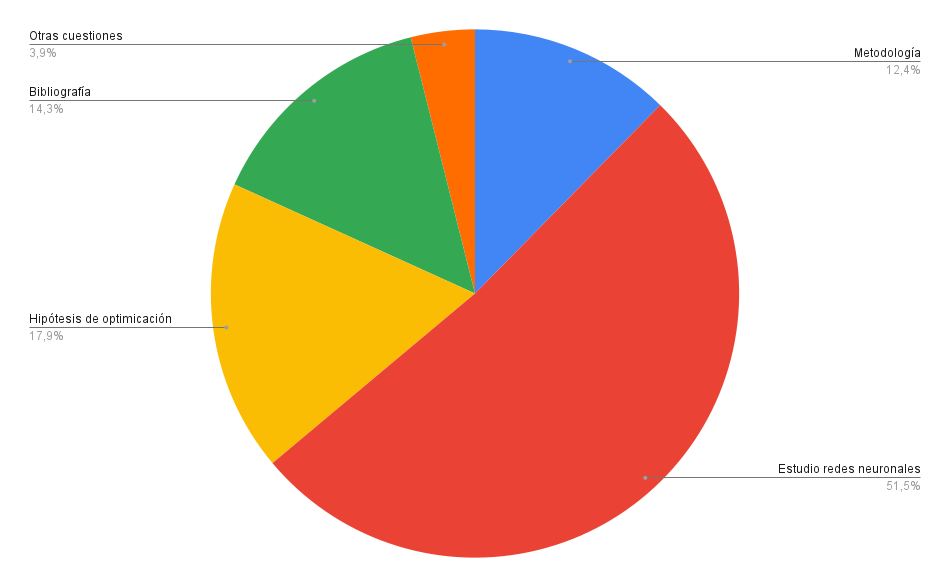
\includegraphics[width=\textwidth]{0-metodologia/chart.png}
     \caption{Sector circular sobre la dedicación a cada hito}
     \label{img:dedicar-hito}
    \end{figure}

\section{Resumen de la metodología}  

Se ha seguido un desarrollo ágil que radica en la resolución de problemas expuestos como historias de usuarios. 
Éstas historias de usuario se formulan en base a los beneficiados, personas bien definidas; se formalizan 
mediante \textit{issues} y entraman los \textit{hitos}, con los que guiar el desarrollo.

Todo esto se puede leer no solo en esta memoria sino también en nuestro repositorio de GitHub \cite{TFG-Estudio-de-las-redes-neuronales}. 
 




